\chapter{The Skein Algebra of the Torus}

\AP{Add some introduction and remark about collaboration.}


\section{Power Sum Elements}

Recall that there is a injective algebra homomorphism $\Lambda \to \ch(A)^+$ which sends the Schur function $s_\lambda$ to the minimal idempotent closure $Q_\lambda$. Use $h_n := Q_{(n)}$ to denote the image of the $n^\textrm{th}$ complete homogeneous symmetric function under this homomorphism. In \AP{MS} the authors import power sum elements from $\Lambda$ to $P_k \in \ch(A)$. The power sum elements have a concrete definition in $\Lambda$, but alternatively they may be defined using an equation of formal power series in the ring $\ch(A)[[t]]$ as
\begin{equation}
\sum_{k=1}^\infty \frac{P_k}{k} t^k = \ln \Bigg( 1 + \sum_{n=1}^\infty h_n t^n \Bigg)
\end{equation}
which writes each $P_k$ in terms of the generators $h_n$. 

Using the Beliakova-Blanchet section $\Gamma: H_n \to BMW_n$, we may emulate this definition to define ``power sum" elements $\tilde{P}_k \in \cd(A)$ by the formal power series equation
\begin{equation}
\sum_{k=1}^\infty \frac{\tilde{P}_k}{k} t^k = \ln \Bigg( 1 + \sum_{n=1}^\infty \tilde{h}_n t^n \Bigg)
\end{equation}
where $\tilde{h}_n := \tilde{Q}_{(n)}$ is the annular closure of the BMW symmetrizers $\tilde{y}_n = \Gamma(y_n)$.

Let's now continue our discussion of Section \ref{sec:relativeannulus} with the following theorem.

\begin{theorem} \label{thm:powersumcommutator}
For any $k \geq 1$, the relation
\begin{equation} \label{eq:powersumcommutator}
e \cdot \tilde{P}_k - \tilde{P}_k \cdot e = (s^k - s^{-k}) (a^k - a^{-k})
\end{equation}
holds. Equivalently,
\begin{equation}
a^i \cdot \tilde{P}_k - \tilde{P}_k \cdot a^i = (s^k - s^{-k}) (a^{k+i} - a^{-k+i})
\end{equation}
for any integer $i$.
\end{theorem}

We will split the proof of this theorem into two technical lemmas.

\begin{lemma} \label{lem:powersumcommutator1}
The relations of Theorem \ref{thm:powersumcommutator} hold if and only if 
\begin{equation} \label{eq:skewcommutator}
e \cdot (\tilde{h}_{n+2} + \tilde{h}_n) - (\tilde{h}_{n+2} + \tilde{h}_n) \cdot e = (sa + s^{-1}a^{-1}) (e \cdot \tilde{h}_{n+1}) - (s^{-1}a + sa^{-1}) (\tilde{h}_{n+1} \cdot e)
\end{equation}
for all integers $n \geq -1$, where $\tilde{h}_0 := 1$ and $\tilde{h}_{-1} := 0$.
\end{lemma}
\begin{proof}
The relations of Theorem \ref{thm:powersumcommutator} may be organized into a single power series equation
\begin{equation} \label{eq:skewcommutator}
\sum_{k=1}^\infty \frac{e \cdot \tilde{P}_k - \tilde{P}_k \cdot e}{k} t^k = \sum_{k=1}^{\infty} \frac {(s^k - s^{-k}) (a^k - a^{-k})}{k} t^k
\end{equation}
in $\ca_\cd [[t]]$. Rewrite this equation as
\begin{equation} \label{eq:powersumcommutator2} 
e \cdot \Bigg( \sum_{k=1}^\infty \tilde{P}_k \Bigg) - \Bigg( \sum_{k=1}^\infty \tilde{P}_k \Bigg) \cdot e = \sum_{k=1}^{\infty} \frac {(sat)^k}{k} + \sum_{k=1}^{\infty} \frac {(s^{-1}a^{-1}t)^k}{k} - \sum_{k=1}^{\infty} \frac {(s^{-1}at)^k}{k} - \sum_{k=1}^{\infty} \frac {(sa^{-1}t)^k}{k}
\end{equation}
We can make sense of the left-hand side by extending the algebra homomorphism $x \mapsto e \cdot (x)$ to an algebra homomorphism of rings of formal power series
\begin{center}
\begin{tikzcd}
\cd(A) \arrow[r, "e \cdot (-)"] \arrow[d, hook] & \ca_\cd \arrow[d, hook] \\
\cd(A)[[t]] \arrow[r, "e \cdot (-)"] & \ca_\cd[[t]]
\end{tikzcd}
\end{center}
and similarly for $(-) \cdot e$. Now for shorthand, define 
\[
H(t) := 1 + \sum_{n=1}^\infty \tilde{h}_n t^n
\]
and recall the Taylor series expansion
\[
-\ln(1-x) = \sum_{k=1}^\infty \frac{x^k}{k}
\]
which is a variation of the Newton-Mercator series. Then the Equation \eqref{eq:skewcommutator} becomes
\begin{equation} \label{eq:powersumcommutator3} 
e \cdot \Big( \ln\big(H(t)\big) \Big) - \Big( \ln \big(H(t)\big) \Big) \cdot e = - \ln(1 - sat) - \ln(1 - s^{-1}a^{-1}t) + \ln(1 - s^{-1}at) + \ln(1 - sa^{-1}t).
\end{equation}
The maps $e \cdot (-)$ and $(-) \cdot e$ commute with the natural logarithm. Use this and other natural log properties to write
\begin{equation}
\ln\Big( e \cdot \big( H(t) \big) \big( 1 - (sa + s^{-1}a^{-1})t + t^2 \big) \Big) = \ln\Big( \big( H(t) \big) \cdot e \big( 1 - (s^{-1}a + sa^{-1})t + t^2 \big) \Big).
\end{equation}
Exponentiating both sides and equating coefficients gives the system of equations defined in the statement of the lemma. Each step of the proof is invertible, and thus the two sets of relations are logically equivalent.
\end{proof}

\begin{lemma}
The relations of Lemma \ref{lem:powersumcommutator1} hold.
\end{lemma}
\begin{proof}
If $n=-1$, the relation we would like to show becomes 
\begin{equation*}
e \cdot \tilde{h}_1 - \tilde{h}_1 \cdot e = \{1\} \left( a - a^{-1} \right)
\end{equation*}
which is just the Dubrovnik skein relation. 

For general values of $n$, the proof is a technical computation using repeated applications of the recursive formula for the $\tilde{h}_n$. Since we will need them here, let's recall the formulas given in Section \ref{sec:relativeannulus}. There are recursive formulas
\begin{align}
[n+1] W_n &= e \cdot \tilde{h}_n + [n] s^{-1} a W_{n-1} + [n] s^{-1} \beta_n a^{-1} W^*_{n-1}, \label{eq:r1} \\
[n+1] W^*_n &= \tilde{h}_n \cdot e + [n] s^{-1} a W^*_{n-1} + [n] s^{-1} \beta_n a W_{n-1}, \label{eq:r2} \\
[n+1] W_n &= \tilde{h}_n \cdot e + [n] s a W_{n-1} + [n] s \bar{\beta}_n a^{-1} W^*_{n-1}, \label{eq:r3} \\
[n+1] W^*_n &= e \cdot \tilde{h}_n + [n] s a^{-1} W^*_{n-1} + [n] s^{-1} \bar{\beta}_n a W_{n-1} \label{eq:r4}
\end{align}
and the ``fundamental relation"
\begin{equation}
e \cdot \tilde{h}_n - \tilde{h}_n \cdot e = \{n\} (a W_{n-1} - a^{-1} W^*_{n-1}). \label{eq:f}
\end{equation}

Start by applying Equation \eqref{eq:f} to the relation of Lemma \ref{lem:powersumcommutator1} to obtain an equivalent relation
\begin{align}\label{eq_perprel4}
\begin{split}
\{n+2\} \left( aW_{n+1} - a^{-1}W^*_{n+1} \right) =& \left( sa+s^{-1}a^{-1} \right) \left( e \cdot \tilde{h}_{n+1} \right) - \left( sa^{-1}+s^{-1}a \right) \left( \tilde{h}_{n+1} \cdot e \right) \\
 & \qquad\qquad\qquad\qquad\qquad\qquad - \{n\}\left( aW_{n-1}-a^{-1}W^*_{n-1} \right).
\end{split}
\end{align}
We will show that the left-hand side of this equation may be reduced to the right-hand side by a series of applications of the recursive formulas, which we will signify with an asterisk $\ast$. 
\begin{eqnarray*}
&& \{n+2\} \left( aW_{n+1} - a^{-1}W^*_{n+1} \right) \\
\overset{\ast}{=}&& \{n+2\} \left( \frac{a}{[n+2]} \left( e \cdot \tilde{h}_{n+1} + [n+1]s^{-1}aW_n + [n+1]s^{-1}\beta_{n+1}a^{-1}W^*_n \right) \right.- \\
&&\left.\qquad\qquad\frac{a^{-1}}{[n+2]} \left( \tilde{h}_{n+1} \cdot e + [n+1]s^{-1}a^{-1}W^*_n + [n+1]s^{-1}\beta_{n+1}aW_n \right) \right)  \\
=&& \left( s - s^{-1} \right) \left( \left( a \cdot \tilde{h}_{n+1} + [n+1]s^{-1}a^2W_n + [n+1]s^{-1}\beta_{n+1}W^*_n \right) \right. \\
&&\qquad\qquad\,\,\,\,\,\left.-\left( \tilde{h}_{n+1} \cdot a^{-1} + [n+1]s^{-1}a^{-2}W^*_n + [n+1]s^{-1}\beta_{n+1}W_n \right)\right) \\
\overset{\ast}{=}&&\left( s-s^{-1} \right) \left( \left( a \cdot \tilde{h}_{n+1} + s^{-2}a \left( [n+2]W_{n+1} - \tilde{h}_{n+1} \cdot e - [n+1]s\bar{\beta}_{n+1}a^{-1}W^*_n \right) \right. \right. \\
&&\qquad\qquad\qquad\qquad\qquad\qquad\qquad\qquad\qquad\qquad\qquad\qquad
+ [n+1]s^{-1}\beta_{n+1}W^*_n \Big)  \\
&&\qquad\qquad\,\,\,\, \left. - \left( \tilde{h}_{n+1} \cdot a^{-1} + s^{-2}a^{-1}\left( [n+2]W^*_{n+1} - e \cdot \tilde{h}_{n+1} - [n+1]s\bar{\beta}_{n+1}aW_n \right) \right. \right. \\
&&\qquad\qquad\qquad\qquad\qquad\qquad\qquad\qquad\qquad\qquad\qquad\qquad\quad\quad
+ [n+1]s^{-1}\beta_{n+1}W_n \Big) \Big) \\
=&&\left( sa + s^{-1}a^{-1} \right) \left( e \cdot \tilde{h}_{n+1} \right) - \left( sa^{-1} + s^{-1}a \right) \left( \tilde{h}_{n+1} \cdot e \right) \\
&+& \left( s^{-1}a^{-1} + s^{-3}a \right) \left( \tilde{h}_{n+1} \cdot e \right) - \left( s^{-1}a + s^{-3}a^{-1} \right) \left( e \cdot \tilde{h}_{n+1} \right) \\
&+& \{n+2\}s^{-2}\left( aW_{n+1} - a^{-1} W^*_{n+1} \right) + \{n+1\}s^{-1}\left( \bar{\beta}_{n+1} - \beta_{n+1} \right) \left( W_n - W^*_n \right).
\end{eqnarray*}

We break the computation here to note that the first two terms in the last line also appear on the right hand side of \eqref{eq_perprel4}. Thus, we would like to prove the following equality:
\begin{eqnarray*}
&-&\{n\} \left( aW_{n-1} - a^{-1}W^*_{n-1} \right) \\
=&& \left( s^{-1}a^{-1} + s^{-3}a \right) \left( \tilde{h}_{n+1} \cdot e \right) - \left( s^{-1}a + s^{-3}a^{-1} \right) \left( e \cdot \tilde{h}_{n+1} \right) \\
&+&\{n+2\}s^{-2}\left( aW_{n+1} - a^{-1} W^*_{n+1} \right) - \{n+1\}s^{-1}\left( \bar{\beta}_{n+1} - \beta_{n+1} \right) \left( W_n - W^*_n \right).
\end{eqnarray*}
We will work the right-hand side of this above equation down to the left-hand side by continuing to apply the same identities. A large number of terms cancel and what remains is the desired relation.
%\pagebreak
\begin{eqnarray*}
&& \left( s^{-1}a^{-1} + s^{-3}a \right) \left( \tilde{h}_{n+1} \cdot e \right) - \left( s^{-1}a + s^{-3}a^{-1} \right) \left( e \cdot \tilde{h}_{n+1} \right) \\
&+& \{n+2\}s^{-2}\left( aW_{n+1} - a^{-1} W^*_{n+1} \right) - \{n+1\}s^{-1}\left( \bar{\beta}_{n+1} - \beta_{n+1} \right) \left( W_n - W^*_n \right) \\
=&& \left( s^{-1}a^{-1} + s^{-3}a \right) \left( \tilde{h}_{n+1} \cdot e \right) - \left( s^{-1}a+s^{-3}a^{-1} \right) \left( e \cdot \tilde{h}_{n+1} \right) \\
&+& [n+2]\left( s^{-1}-s^{-3} \right) \left(aW_{n+1} - a^{-1}W^*_{n+1} \right) \\
&+& [n+1]\left( 1-s^{-2} \right) \left( \bar{\beta}_{n+1}-\beta_{n+1} \right) \left(W_n - W^*_n \right) \\
=&& s^{-1}a\left( [n+2]W_{n+1} - e \cdot \tilde{h}_{n+1} \right) \\
&+& s^{-3}a^{-1}\left( [n+2]W^*_{n+1} - e \cdot \tilde{h}_{n+1} \right) \\
&-& s^{-3}a\left( [n+2]W_{n+1} - \tilde{h}_{n+1} \cdot e \right) \\
&-& s^{-1}a^{-1}\left( [n+2]W^*_{n+1} - \tilde{h}_{n+1} \cdot e \right) \\
&+& [n+1]\left( 1-s^{-2} \right) \left( \bar{\beta}_{n+1} -\beta_{n+1} \right) \left( W_n - W^*_n \right) \\
\overset{\ast}{=}&& s^{-1}a\left( [n+1]s^{-1}aW_n + [n+1]s^{-1}\beta_{n+1}a^{-1}W^*_n \right) \\
&+& s^{-3}a^{-1}\left( [n+1]sa^{-1}W^*_n + [n+1]s\bar{\beta}_{n+1}aW_n \right) \\
&-&s^{-3}a\left( [n+1]saW_n + [n+1]s\bar{\beta}_{n+1}a^{-1}W^*_n \right) \\
&-& s^{-1}a^{-1}\left( [n+1]s^{-1}a^{-1}W^*_n + [n+1]s^{-1}\beta_{n+1}aW_n \right) \\
&+& [n+1]\left(1-s^{-2} \right) \left( \bar{\beta}_{n+1} - \beta_{n+1} \right) \left( W_n - W^*_n \right)\\
=&& [n+1]\left( s^{-2}a^2W_n + s^{-2}\beta_{n+1}W^*_n + s^{-2}a^{-2}W^*_n + s^{-2}\bar{\beta}_{n+1}W_n - s^{-2}a^{2}W_n \right. \\
&&\qquad\quad \left. - s^{-2}\bar{\beta}_{n+1}W^*_n - s^{-2}a^{-2}W^*_n - s^{-2}\beta_{n+1}W_n + \bar{\beta}_{n+1}W_n - \bar{\beta}_{n+1}W^*_n - \beta_{n+1}W_n \right. \\
&&\qquad\quad \left. + \beta_{n+1}W^*_n - s^{-2}\bar{\beta}_{n+1}W_n + s^{-2}\bar{\beta}_{n+1}W^*_n + s^{-2}\beta_{n+1}W_n - s^{-2}\beta_{n+1}W^*_n \right) \\
=&& [n+1]\left( \bar{\beta}_{n+1} - \beta_{n+1} \right) \left( W_n - W^*_n \right) \\
=&& \left( \bar{\beta}_{n+1} - \beta_{n+1} \right) \left( \left( [n+1]W_n \right) - \left( [n+1]W^*_n \right) \right) \\
\overset{\ast}{=}&& \left( \bar{\beta}_{n+1} - \beta_{n+1} \right) \left( \left( e \cdot \tilde{h}_{n} + [n]s^{-1}aW_{n-1} + [n]s^{-1}\beta_{n}a^{-1}W^*_{n-1} \right) \right. \\
&& \qquad\qquad\qquad\qquad \left. -\left( e \cdot \tilde{h}_{n} + [n]sa^{-1}W^*_{n-1} + [n]s\bar{\beta}_{n}aW_{n-1} \right) \right) \\
=&& \left( \bar{\beta}_{n+1} - \beta_{n+1} \right) \left( [n]\left( s^{-1} - s\bar{\beta}_{n} \right) aW_{n-1} - [n]\left( s-s^{-1}\beta_{n} \right) a^{-1}W^*_{n-1} \right) \\
=&& [n]\left(\bar{\beta}_{n+1} - \beta_{n+1} \right) \left( s - s^{-1}\beta_{n} \right) \left( aW_{n-1} - a^{-1}W^*_{n-1} \right) \\
=&-& \{n\}\left( aW_{n-1} - a^{-1}W^*_{n-1} \right).
\end{eqnarray*}
Where the last equality follows from a quick computation in the base ring. This completes the proof.
\end{proof}

This next theorem follows directly from Equation \eqref{eq:skewcommutator}, which makes it equivalent to Theorem \ref{thm:powersumcommutator} in some sense. This expresses the left $\cd(A)$-action on $\ca_\cd$ in terms of the right action, and vice versa. This implies a commutation relation for the closures of the BMW symmetrizers in terms of either the elements of the set $\{\tilde{h}_j \cdot a^i \}_{j, i}$ or $\{ a^i \cdot \tilde{h}_j \}_{j, i \geq 0}$ which are subsets of the bases $\{ Q_\lambda \cdot a^i \}_{i \geq 0, \lambda}$ and $\{ a^i \cdot Q_\lambda \}_{i \geq 0, \lambda}$ of $\ca_\cd$, respectively. These supersets are bases since $\ca_\cd = \cd(A)[a, a^{-1}]$ as algebras in the category of left $\cd(A)$-modules and because the map defined by $Q_\lambda \cdot a^i \mapsto a^i \cdot Q_\lambda$ is an invertible algebra homomorphism. 

\begin{theorem} \label{prop:hncommutator}
For any $n \geq 1$, the relations
\begin{equation}
\tilde{h}_n \cdot e = \sum_{i=0}^n d_i (e \cdot \tilde{h}_{n-i})
\end{equation}
and
\begin{equation}
e \cdot \tilde{h}_n = \sum_{i=0}^n \bar{d}_i (\tilde{h}_{n-i} \cdot e)
\end{equation}
hold in $\ca_\cd$, where
\begin{align*}
d_0 & = 1, \\
d_i & = \sum_{l=0}^{i-1} (1 - s^2) s^{2l-i} a^{i-2l} + (1 - s^{-2}) s^{i-2l} a^{2l-i} \qquad \forall i \geq 1, \\
\bar{d}_i & = \sum_{l=0}^{i-1} (1 - s^{-2}) s^{i-2l} a^{i-2l} + (1 - s^{2}) s^{2l-i} a^{2l-i} \qquad \forall i \geq 1.
\end{align*}
Equivalently,
\begin{equation}
e \cdot \tilde{h}_n - \tilde{h}_n \cdot e = \sum_{i=1}^n \bar{d}_i (\tilde{h}_{n-i} \cdot e)
\end{equation}
or 
\begin{equation}
\tilde{h}_n \cdot e - e \cdot \tilde{h}_n = \sum_{i=1}^n d_i (e \cdot \tilde{h}_{n-i}).
\end{equation}
\end{theorem}
\begin{proof}
The formula for the $d_i$ were discovered experimentally by coding a solver using the SymPy package in Python. The second equation is just the mirror map applied to the first equation, so we will just prove the first equation.

The idea of the proof depends on a reformulation of Equation \eqref{eq:skewcommutator} as
\[
\tilde{h}_n \cdot e = e \cdot \tilde{h}_n - ( s a + s^{-1} a^{-1} ) ( e \cdot \tilde{h}_{n-1} ) + e \cdot \tilde{h}_{n-2} + ( s^{-1} a + s a^{-1} ) \tilde{h}_{n-1} \cdot e - \tilde{h}_{n-2} \cdot e
\]
and a recursive application of this formula to its last two terms on the right-hand side of the equation. 

The case of $n=0$ is trivial. For $n=1$, just apply the Kauffman skein relation. Now assume the induction hypothesis, that the formula in the statement is true for all $k \leq n-1$. Then apply this assumption to Equation \eqref{eq:skewcommutator}:
\begin{align*}
\tilde{h}_n \cdot e &= e \cdot \tilde{h}_n - ( s a + s^{-1} a^{-1} ) ( e \cdot \tilde{h}_{n-1} ) + e \cdot \tilde{h}_{n-2} + ( s^{-1} a + s a^{-1} ) ( \tilde{h}_{n-1} \cdot e ) - \tilde{h}_{n-2} \cdot e \\
&= e \cdot \tilde{h}_n - ( s a + s^{-1} a^{-1} ) ( e \cdot \tilde{h}_{n-1} ) + e \cdot \tilde{h}_{n-2} + ( s^{-1} a + s a^{-1} ) \sum_{i=0}^{n-1} d_i (e \cdot \tilde{h}_{n-1-i}) \\
&\qquad\qquad\qquad\qquad\qquad\qquad\qquad\qquad\qquad\qquad\qquad\qquad\qquad\qquad - \sum_{i=0}^{n-2} d_i (e \cdot \tilde{h}_{n-2-i}) \\
&= e \cdot \tilde{h}_n + d_1 ( e \cdot \tilde{h}_{n-1} ) + ( s^{-1} a + s a^{-1} ) \sum_{i=1}^{n-1} d_i (e \cdot \tilde{h}_{n-1-i}) - \sum_{i=1}^{n-2} d_i (e \cdot \tilde{h}_{n-2-i}) \\
&= e \cdot \tilde{h}_n + d_1 ( e \cdot \tilde{h}_{n-1} ) + ( s^{-1} a + s a^{-1} ) \sum_{i=0}^{n-2} d_{i+1} (e \cdot \tilde{h}_{n-2-i}) - \sum_{i=1}^{n-2} d_i (e \cdot \tilde{h}_{n-2-i}) \\
&= e \cdot \tilde{h}_n + d_1 ( e \cdot \tilde{h}_{n-1} ) + ( s^{-1} a + s a^{-1} ) d_1 ( e \cdot \tilde{h}_{n-2} ) \\
&\qquad\qquad\qquad\qquad\qquad\qquad\qquad\qquad\quad\quad+ \sum_{i=1}^{n-2} \big( ( s^{-1} a + s a^{-1} ) d_{i+1} - d_i \big) (e \cdot \tilde{h}_{n-2-i}). \\
\end{align*}
It is a straightforward computation to show that $( s^{-1} a + s a^{-1} ) d_1 = d_2$:
\begin{align*}
( s^{-1} a + s a^{-1} ) d_1 &= ( s^{-1} a + s a^{-1} ) \big( ( 1 - s^2 ) s^{-1} a + ( 1 + s^{-2} ) s a^{-1} \big) \\
&= ( 1 - s^2 ) s^{-2} a^2 + (1 - s^{-2} ) s^0 a^0 + ( 1 - s^2 ) s^0 a^0 + ( 1 - s^{-2} ) s^2 a^{-2} \\
&= d_2.
\end{align*}
It's slightly more tedious to show that $( s^{-1} a + s a^{-1} ) d_{i+1} - d_i = d_{i+2}$ for all $i \geq 1$:
\begin{eqnarray*}
&&( s^{-1} a + s a^{-1} ) d_{i+1} - d_i \\
=&& ( s^{-1} a + s a^{-1} ) \sum_{l=0}^{i} (1 - s^2) s^{2l-i} a^{i-2l} + (1 - s^{-2}) s^{i-2l} a^{2l-i} \\
&-& \sum_{l=0}^{i-1} (1 - s^2) s^{2l-(i-1)} a^{(i-1)-2l} + (1 - s^{-2}) s^{(i-1)-2l} a^{2l-(i-1)} \\
=&& \sum_{l=0}^{i} (1 - s^2) s^{2l-(i+1)} a^{(i+1)-2l} + (1 - s^{-2}) s^{(i+1)-2l} a^{2l-(i+1)} \\
&+& \sum_{l=0}^{i} (1 - s^2) s^{2l-(i-1)} a^{(i-1)-2l} + (1 - s^{-2}) s^{(i-1)-2l} a^{2l-(i-1)} \\
&-& \sum_{l=0}^{i-1} (1 - s^2) s^{2l-(i-1)} a^{(i-1)-2l} + (1 - s^{-2}) s^{(i-1)-2l} a^{2l-(i-1)} \\
=&& \sum_{l=0}^{i} (1 - s^2) s^{2l-(i+1)} a^{(i+1)-2l} + (1 - s^{-2}) s^{(i+1)-2l} a^{2l-(i+1)} \\
&+& (1 - s^2) s^{i+1} a^{-1-i} + (1 - s^{-2}) s^{-1-i} a^{i+1} \\
=&& d_{i+2}.
\end{eqnarray*}
This completes the proof of the statement. 
\end{proof}

\begin{remark}
There exists an algebra homomorphism from $\cd(A)$ to the ring of symmetric functions $\Lambda_R$ (see \AP{chapter whatever}). Conjecturally, this map is an isomorphism, which would imply that the sets $\{ \tilde{h}_\lambda \cdot a^i \}_{\lambda, i}$ and $\{ a^i \cdot \tilde{h}_\lambda \}_{\lambda, i}$ over integers $i$ and partitions $\lambda$, where $\tilde{h}_\lambda := \tilde{h}_{\lambda_1} \cdots \tilde{h}_{\lambda_r}$, form bases of $\ca_\cd = \cd(A)[a, a^{-1}]$ \AP{or is this already known separately somehow?}. If so, then Theorem \ref{prop:hncommutator} provides transition formulas between these two bases, and therefore giving a full description of $\ca_\cd$ as a $\cd(A)$-$\cd(A)$-bimodule. 
\end{remark}

As an aside, one might expect similar formulas to hold in the HOMFLYPT case. To our knowledge, there is no HOMFLYPT analogue of Theorem \ref{prop:hncommutator} written down in the literature. Let's do that here. 

\begin{lemma} \label{lem:homfly1}
For all integers $n$, the following relation holds in $\ca_\ch$
\begin{equation}
e \cdot h_n - h_n \cdot e = s a \cdot h_{n-1} - h_{n-1} \cdot  s^{-1} a
\end{equation}
where we use the convention $h_0 = 1$ and $h_n = 0$ if $n < 0$. 
\end{lemma}
\begin{proof}
Recall the power sum elements $P_k$ satisfy the power series equation
\begin{equation} \label{def:Pk}
\sum_{k=1}^\infty \frac{P_k}{k} x^k = \ln \Big( \sum_{n=0}^\infty h_n x^n \Big)
\end{equation}
By \cite[Theorem 4.2]{Mor02b}\AP{fix}, the power sum elements satisfy a commutation relation in $\ca_\ch$
\begin{equation}
e \cdot P_k - P_k \cdot e = (s^{k} - s^{-k}) a^k
\end{equation} 
which may be rephrased as a power series equation 
\[
e \cdot \Big( \sum_{k=1}^\infty P_k x^k \Big) - \Big( \sum_{k=1}^\infty P_k x^k \Big) \cdot e = \sum_{k=1}^\infty s^k a^k - \sum_{k=1}^\infty s^{-k} a^k.
\]
On the left-hand side, use the defining equation \eqref{def:Pk}. Use the power series formulation of natual log on the right-hand side. So we have
\[
\ln \Bigg( e \cdot \Big( \sum_{k=0}^\infty h_k x^k \Big) \Bigg) - \ln \Bigg( \Big( \sum_{k=0}^\infty h_k x^k \Big) \cdot e \Bigg) = \ln ( 1 - s a x ) - \ln ( 1 - s^{-1} a x ).
\]
After moving terms around, using properties of natural log, and exponentiating both sides, we arrive at the equation
\[
\Big( \sum_{n=0}^\infty (h_n \cdot e ) x^n \Big) ( 1 - s a x ) = \Big( \sum_{n=0}^\infty ( e \cdot h_n ) x^k \Big) ( 1 - s^{-1} a x )
\]
which implies the statement of the lemma.
\end{proof}

Recall that the algebra $\ca_\ch$ is equal to the Laurent polynomial ring $\ch(A)^+[a, a^{-1}]$. Under the isomorphism between $\ch(A)^+$ and the ring of symmetric functions $\Lambda_R$, the $h_n$ identify with the complete homogeneous symmetric functions. It is well-known that ordered monomials in the complete homogeneous symmetric functions form a basis of $\Lambda$, hence the sets $\{h_\lambda \cdot a^i \}_{\lambda, i}$ and $\{a^i \cdot h_\lambda \}_{\lambda, i}$ over integers $i$ and partitions $\lambda$, where $h_\lambda := h_{\lambda_1} \cdots h_{\lambda_r}$, form bases of $\ca_\ch$. The following theorem gives transition formulas between these two bases. 

\begin{theorem} \label{prop:homfly2}
The Hecke symmetrizers $h_n$ satisfy the equations
\[
h_n \cdot e = e \cdot h_n + ( 1 - s^2 ) \sum_{l=1}^{n} s^{-l} ( a^l \cdot h_{n-l} )
\]
and
\[
e \cdot h_n = h_n \cdot e + (1 - s^{-2} ) \sum_{l=1}^{n} s^l ( h_{n-l} \cdot a^l ).
\]
\end{theorem}
\begin{proof}
We will prove the first equality. The second is completely analagous. Proceed by induction. When $n=1$, the statement follows from the HOMFLY skein relation. 

We can rearrange the terms of Lemma \ref{lem:homfly1} to get
\begin{equation} \label{eq:homfly1b}
h_n \cdot e = e \cdot h_n + s^{-1} a ( h_{n-1} \cdot e ) - s a ( e \cdot h_{n-1} ).
\end{equation}
By the induction hypothesis,
\begin{align*}
h_n \cdot e & = e \cdot h_n + s^{-1} a ( h_{n-1} \cdot e ) - s a ( e \cdot h_{n-1} ) \\
& = e \cdot h_n + s^{-1} a \Big( e \cdot h_{n-1} + ( 1 - s^2 ) \sum_{j=1}^{n-1} s^{-j} a^j ( e \cdot h_{n-1-j} ) \Big) - s a ( e \cdot h_{n-1} ) \\
& = e \cdot h_n + ( s^{-1} - s ) a ( e \cdot h_{n-1} ) + ( 1 - s^2 ) \sum_{j=1}^{n-1} s^{-j-1} a^{j+1} ( e \cdot h_{n-1-j} ) \\ 
& = e \cdot h_n + ( 1 - s^2 ) s^{-1} a ( e \cdot h_{n-1} ) + ( 1 - s^2 ) \sum_{j=1}^{n-1} s^{-(j+1)} a^{j+1} ( e \cdot h_{n-(j+1)} ) \\
&= e \cdot h_n + ( 1 - s^2 ) \sum_{l=1}^{n} s^{-l} a^{l} ( e \cdot h_{n-l} )
\end{align*}
where the last equality follows from the substitution $j=l+1$. 
\end{proof}


\section{A Presentation of $\cd(T^2)$}

In this section we will demonstrate the value of the elements $\tilde{P}_k$  by showing that the skein algebra $\cd(T^2)$ admits a very simple presentation. First things first, let's define the generators. Recall that given an extended rational number $r$, there is a (homotopically) distinct oriented simple closed curve on the flat torus $T^2$ with rational slope $r$, and hence a smooth embedding of the annulus 
\[
\iota_r: A \to T^2
\]
into tubular neighborhood of the curve. This induces an algebra homomorphism
\[
\cd(\iota_r): \cd(A) \to \cd(T^2)
\]
on the level of skein algebras. Any knot in $\cd(T^2)$ is contained in the image of some $\cd(\iota_r)$. Since $\cd$ is an unoriented skein theory, let's only consider $r \geq 0$ to avoid redundancy due to the choice of orientations. Given any equivalence class $\xx = (a, b)$ in $\Z^2 / \langle \xx = - \xx \rangle$ with $k := \gcd(a, b)$, define the element
\[
\tilde{P}_\xx := \cd\big(\iota_{|a/b|}\big)(\tilde{P}_k)
\]
to be the embedding of the ``power sum" element $\tilde{P}_k$ into this tubular neighborhood. Let's state the main theorem of the paper.

\begin{theorem}
The skein algebra $\cd(T^2)$ is presented by generators 
\[
\{ \tilde{P}_\xx \mid \xx \in \Z^2 / \langle \xx = - \xx \rangle \}
\]
and relations
\begin{equation} \label{eq:mainrelations}
[\tilde{P}_\xx, \tilde{P}_\yy] = (s^{\det(\xx, \yy)} - s^{-\det(\xx, \yy)}) (\tilde{P}_{\xx + \yy} - \tilde{P}_{\xx - \yy}).
\end{equation}
\end{theorem}

\begin{corollary}
The linear span of the set $\{ \tilde{P}_\xx \mid \xx \in \Z^2 / \langle \xx = - \xx \rangle \}$ is a Lie algebra, and  $\cd(T^2)$ is its universal enveloping algebra. 
\end{corollary}

The full proof of this theorem may be found in the collaboration \AP{MPS}. Here, we will be focused on showing that the generators satisfy the relations given in the presentation. We formulate this as a proposition.
\begin{proposition}
The following special cases of Equation \eqref{eq:mainrelations} hold
\begin{align}
[\tilde{P}_{1, 0}, \tilde{P}_{0, n}] &= (s^n - s^{-n}) (\tilde{P}_{1, n} - \tilde{P}_{1, -n}) \label{eq:perprelations} \\
[\tilde{P}_{1, 0}, \tilde{P}_{1, n}] &= (s^n - s^{-n}) (\tilde{P}_{2, n} - \tilde{P}_{0, n}) \label{eq:angledrelations}
\end{align}
for any $n \geq 1$. Furthermore, these relations generate all of the relations defined by Equation \eqref{eq:mainrelations}.
\end{proposition}

Equation \eqref{eq:perprelations} is the image of Equation \eqref{eq:powersumcommutator} under the wiring of $\ca_\cd$ into $\cd(T^2)$ depicted below.

\AP{Picture of wiring.}

We will not give the proof of Equation \eqref{eq:angledrelations} here \AP{This part of the proof was finished before I started working on the project}, but it may be found in \AP{MPS}. The idea given there is similar to the idea for the proof of Equation \eqref{eq:perprelations}: first show a similar relation holds in the skein algebra of the annulus relative to two points $\cd(A, [2])$ via a brute force computation, and then Equation \eqref{eq:angledrelations} is the image of this relation under a simple wiring into $\cd(T^2)$. 

What's left for us to show here is the second statement of the proposition, that Equations \eqref{eq:perprelations} and \eqref{eq:angledrelations} imply Equation \eqref{eq:mainrelations}. We will devote the rest of this section to doing so, starting with two technical lemmas and ending with Proposition \ref{lemma_allfromsome}. 

We use the notation
\begin{align*} 
d(\xx, \yy) &:= \det\left[\xx\,\, \yy\right] \quad \quad \,\,  \textrm{for } \xx, \yy \in \Z^2, \\
d(\xx) &:= gcd(m,n) \quad \quad \textrm{when } \xx = (m,n).
\end{align*} 
We will also use the following terminology: 
\[
(\xx,\yy) \in \Z^2 \times \Z^2 \textrm{ is \emph{good} if  } [\tilde{P}_\xx,\tilde{P}_\yy] = \{d(\xx,\yy)\} \left( \tilde{P}_{\xx+\yy}-\tilde{P}_{\xx-\yy} \right).
\]

\begin{remark}\label{remark_goodsymmetry}
Note that because $\tilde{P}_{\xx}=\tilde{P}_{-\xx}$, if $(\xx, \yy)$ is good, then the pairs $(\pm\xx, \pm\yy)$ are good as well. 
\end{remark}

The idea of the proof is to induct on the absolute value of the determinant of the matrix with columns $\xx$ and $\yy$. To induct, we write $\xx = \aab + \bb$ for carefully chosen vectors $\aab, \bb$ and then use the following lemma. 
%We have indicated an example choice of the vectors $\xx$, $\yy$, $\aab$ and $\bb$ in Figure \ref{fig_vectors}. 
%\AP{Did we want to include a figure?} \PS{We only included it because the referee asked for it, so let's ignore it for now.}\\
%It is easy to see that Lemma \ref{lemma_trueforab} applies to the vectors in this example.

\begin{lemma}\label{lemma_trueforab}
	Assume $\aab + \bb = \xx$ and that $(\aab,\bb)$ is good. Further assume that the five pairs of vectors $(\yy, \aab)$, $(\yy, \bb)$, $(\yy+\aab,\bb)$, $(\yy+\bb,\aab)$, and $(\aab-\bb, \yy)$, are good. Then the pair $(\xx,\yy)$ is good.
\end{lemma}
\begin{proof}
We  use the Jacobi identity and the goodness assumptions to compute
	\begin{eqnarray*}
&-&\{d(\aab, \bb)\} [\tilde{P}_{\aab+\bb}, \tilde{P}_y] + \{d(\aab, \bb)\} [\tilde{P}_{\aab-\bb}, \tilde{P}_y] \\
=&-&[[\tilde{P}_{\aab}, \tilde{P}_{\bb}], \tilde{P}_{\yy}] \\
=&&[[\tilde{P}_{\yy}, \tilde{P}_{\aab}], \tilde{P}_{\bb}] + [[\tilde{P}_{\bb}, \tilde{P}_y], \tilde{P}_{\aab}] \\
=&&\{d(\yy, \aab)\} [\tilde{P}_{\yy+\aab} - \tilde{P}_{\yy-\aab}, \tilde{P}_{\bb}] + \{d(b,y)\} [\tilde{P}_{\bb+\yy} - \tilde{P}_{\bb-\yy}], \tilde{P}_{\aab}] \\
=&&\{d(\yy,\aab)\} \left( \{d(\yy+\aab, \bb)\} \left( \tilde{P}_{\yy+\aab+\bb} - \tilde{P}_{\yy+\aab-\bb} \right) \right. \\
&& \left. \qquad\qquad -\{d(\yy-\aab,\bb)\} \left( \tilde{P}_{\yy-\aab+\bb} - \tilde{P}_{\yy-\aab-\bb} \right) \right) \\
&+&\{d(\bb,\yy)\} \left( \{d(\bb+\yy, \aab)\} \left( \tilde{P}_{\bb+\yy+\aab} - \tilde{P}_{\bb+\yy-\aab} \right) \right. \\
&& \left. \qquad\qquad -\{d(\bb-\yy, \aab)\} \left( \tilde{P}_{\bb-\yy+\aab} - \tilde{P}_{\bb-\yy-\aab} \right) \right) \\
=&& \left( \{d(\yy,\aab)\} \{d(\yy+\aab,\bb)\} + \{d(\bb,\yy)\} \{d(\bb+\yy,\aab)\} \right) \tilde{P}_{\aab+\bb+\yy} \\
&+& \left( \{d(\yy,\aab)\} \{d(\yy-\aab,\bb)\} - \{d(\bb,\yy)\} \{d(\bb-\yy,\aab)\} \right) \tilde{P}_{\aab+\bb-\yy} \\
&-& \left( \{d(\yy,\aab)\} \{d(\yy+\aab,\bb)\} - \{d(\bb,\yy)\} \{d(\bb-\yy,\aab)\} \right) \tilde{P}_{\aab-\bb+\yy} \\
&-& \left( \{d(\yy,\aab)\} \{d(\yy-\aab,\bb)\} + \{d(\bb,\yy)\} \{d(\bb+\yy,\aab)\} \right) \tilde{P}_{\aab-\bb-\yy} \\
=:&& c_1 \tilde{P}_{\aab+\bb+\yy} + c_2 \tilde{P}_{\aab+\bb-\yy} - c_3 \tilde{P}_{\aab-\bb+\yy} - c_4 \tilde{P}_{\aab-\bb-\yy}.
	\end{eqnarray*}
Using some simple algebra, we can show
	\begin{eqnarray*}
c_1 \,\,\, =& &  \{d(\yy,\aab)\} \{d(\yy+\aab,\bb)\} + \{d(\bb,\yy)\} \{d(\bb+\yy,\aab)\} \\
=&& \{d(\yy,\aab)+d(\yy+\aab,\bb)\}^+ - \{d(\yy,\aab)-d(\yy+\aab,\bb)\}^+ \\
&+& \{d(\bb,\yy)+d(\bb+\yy,\aab)\}^+ - \{d(\bb,\yy)-d(\bb+\yy,\aab)\}^+  \\
=&& \{d(\yy,\aab+\bb)+d(\aab,\bb)\}^+ - \{d(\yy,\aab-\bb)-d(\aab,\bb)\}^+ \\
&+& \{d(\yy,\aab-\bb)-d(\aab,\bb)\}^+ - \{d(\aab,\bb)-d(\yy,\aab+\bb)\}^+ \\
=&& \{d(\aab,\bb)+d(\yy,\aab+\bb)\}^+ - \{d(\aab,\bb)-d(\yy,\aab+\bb)\}^+ \\
=&& \{d(\aab,\bb)\} \{d(\yy,\aab+\bb)\} \\
=&& - \{d(\aab,\bb)\} \{d(\xx,\yy)\}.
	\end{eqnarray*}
Similar computations for the other $c_i$ show that 
	\begin{align}
\frac{1}{\{d(\aab,\bb)\}}[[\tilde{P}_\aab,\tilde{P}_\bb],\tilde{P}_\yy] &=  \frac{-1}{\{d(\aab,\bb)\}} \left( c_1 \tilde{P}_{\aab+\bb+\yy} + c_2 \tilde{P}_{\aab+\bb-\yy} - c_3 \tilde{P}_{\aab-\bb+\yy} - c_4 \tilde{P}_{\aab-\bb-\yy}\right) \notag\\ 
&=  \{d(\xx,\yy)\} \left( \tilde{P}_{\xx+\yy} - \tilde{P}_{\xx-\yy} \right) 
-\{d(\aab-\bb,\yy)\} \left( \tilde{P}_{\aab-\bb+\yy} - \tilde{P}_{\aab-\bb-\yy} \right)\notag \\
&= \{d(\xx,\yy)\} \left( \tilde{P}_{\xx+\yy} - \tilde{P}_{\xx-\yy} \right) 
- [\tilde{P}_{\aab-\bb},\tilde{P}_\yy]. \label{eq:astep}
	\end{align}
	Since the pair $(\aab,\bb)$ is good, we have 
\begin{equation}\label{eq:added}
[\tilde{P}_{\aab}, \tilde{P}_{\bb}] = \{d(\aab, \bb )\} \big( \tilde{P}_{\xx} - \tilde{P}_{\aab-\bb} \big).
\end{equation}
Finally, combining equations \eqref{eq:added} and \eqref{eq:astep} shows that the pair $(\xx,\yy)$ is good.
\end{proof}

Now we'll need to prove the following elementary lemma (which is a slight modification of \cite[Lemma 1]{FG00} \AP{fix}). This is used to make a careful choice of vectors $\aab, \bb$ so that the previous lemma can be applied. 

\begin{lemma}\label{lemma_diophantine}
	Suppose $p,q \in \N$ are relatively prime with $q < p$. Then there exist $u,v,w,z \in \Z$ such that the following conditions hold:
	\begin{eqnarray*}
	0 \,<\, u, w &<& p, \\
	\det\left[ \begin{array}{cc} u&w\\v&z\end{array}\right] &=& 1, \\
	\left[ \begin{array}{cc} u&w\\v&z\end{array}\right]\left[\begin{array}{c}1\\1\end{array}\right] &=& \left[ \begin{array}{c}p\\q\end{array}\right].
	\end{eqnarray*}
\end{lemma}
\begin{proof}
	Since $p$ and $q$ are relatively prime, there exist $a,b \in \Z$ with $ bq - ap = 1$. This solution can be modified to give another solution $a' = a + q$ and $b' = b + p$, so we may assume $0 \leq b < p$. We then define 
	\[
	u=b,\quad v=a,\quad w=p-b,\quad z=q-a.
	\]
	By definition, $u,v,w,z$ satisfy $u + w = p$ and $v + z = q$, and the inequalities $0 \leq b < p$ and $p > 1$ imply the condition $0 < u, w < p$. To finish the proof, we compute
	\[
	uz - wv = b(q-a) - a(p-b) = bq - ap = 1.
	\]
\end{proof}

\begin{remark}\label{remark_gl2z}
The mapping class group of a (smooth) surface $\Sigma$ is the group of isotopy classes of (smooth) orientation-preserving homeomorphisms $\Sigma \to \Sigma$. Any skein algebra $\cs_X(\Sigma)$ is acted on by the mapping class group of $\Sigma$: the mapping class group is generated by Dehn twists on $\Sigma$ and may be extended trivially onto $\Sigma \times I$, which induce algebra endomorphisms on the skein algebra due to functoriality of $\cs_X(-)$. Thus, there is an $SL_2(\Z)$-action on $\cd(T^2)$ and is such that $g \cdot \tilde{P}_\xx = \tilde{P}_{g\xx}$ for any $g \in \SL_2(\Z)$. One could choose to extend this to an action of the \textit{extended} mapping class group of $\Sigma$ (that is, to include orientation-reversing diffeomorphisms) so that $GL_2(Z)$ acts on $\cd(T^2)$. If matrices of determinant $-1$ are to act on $\cd(T^2)$ in the same way as before, then they will induce anti-linear algebra anti-homomorphisms on $\cd(T^2)$. One could turn these into honest algebra homomorphisms by composing with the mirror map (note that $\tilde{P}_\xx$ is fixed by the mirror map since the BMW symmetrizers are). It will be important that the orbits of this action on the $\tilde{P}_{\xx}$ are the fibers of the assignment $\tilde{P}_{\xx} \mapsto d(\xx)$ (which is essentially the statement of Lemma \ref{lemma_diophantine}). In other words, up to the action of $GL_2(\Z)$, vectors in $\Z^2$ are classified by the GCD of their entries.
\end{remark}

\begin{proposition}\label{lemma_allfromsome}
Suppose $A$ is an algebra with elements $\tilde{P}_\xx$ for $\xx \in \Z^2/\langle -\xx = \xx \rangle$ that satisfy equations \eqref{eq:perprelations} and \eqref{eq:angledrelations}. Furthermore, suppose that there is a $\GL_2(\Z)$-action on $A$ so that $g \cdot \tilde{P}_\xx = \tilde{P}_{g \xx}$ for any $g \in \GL_2(\Z)$. Then, any pair $(\xx, \yy)$ is a good pair. 
\end{proposition}
\begin{proof}
	The proof proceeds by induction on $\lvert d(\xx,\yy)\rvert $, and the base case $\lvert d(\xx,\yy)\rvert = 1$ is immediate from Remark \ref{remark_gl2z} and the assumption \eqref{eq:perprelations} for $\xx = (1,0)$ and $\yy = (0,1)$. We now make the following inductive assumption:
	\begin{equation}\label{assumption1} 
	\textrm{For all } \xx',\yy' \in \Z^2\textrm{ with } \lvert d(\xx',\yy')\rvert < \lvert d(\xx,\yy) \rvert, \textrm{ the pair } (\xx',\yy') \textrm{ is good.}
	\end{equation}
	We would like to show that $[\tilde{P}_{\xx},\tilde{P}_{\yy}] = \{d(\xx,\yy)\} \big( \tilde{P}_{\xx + \yy} - \tilde{P}_{\xx-\yy} \big)$. By Remark \ref{remark_gl2z}, we may assume
	\[
	\yy = \begin{bmatrix}0\\r\end{bmatrix},\quad \xx = \begin{bmatrix}p\\q\end{bmatrix},\quad d(\xx) \leq d(\yy),\quad 0 \leq q < p.
	\]
	
	If $p=1$, then this equation follows from Equation \eqref{eq:angledrelations}, so we may also assume $p > 1$. Furthermore, we may assume that $r>0$ by Remark \ref{remark_goodsymmetry}. 

	We will now show that if either $d(\xx)=1$ or $d(\yy)=1$, then $(\xx,\yy)$ is good. By symmetry of the above construction of $\xx$ and $\yy$, we may assume $d(\xx)=1$, which immediately implies $q>0$. Furthermore, we may now assume that $r>1$ by assuming Equation \eqref{eq:angledrelations}. We apply Lemma \ref{lemma_diophantine} to $p, q$ to obtain  $u,v,w,z \in \Z$ satisfying 
	\begin{equation}\label{assumption1.49}
	uz - vw = 1,\quad uq - vp = 1,\quad u + w = p,\quad v + z = q,\quad 0 < u,w < p.
	\end{equation}
	We then define vectors $\aab$ and $\bb$ as follows:
	\begin{equation}\label{assumption1.9}
	\aab := \begin{bmatrix}  u\\ v\end{bmatrix},\quad 
	\bb := \begin{bmatrix} w\\ z\end{bmatrix},
	\quad \aab + \bb = \xx,\quad d(\aab, \bb) = 1. %,\quad 0 < d(\xx)u,d(\xx)w < p
	\end{equation}

	Using Lemma \ref{lemma_trueforab} and Assumption (\ref{assumption1}), it is sufficient to show that each of $\lvert d(\aab, \bb) \rvert$, $\lvert d(\yy,\bb) \rvert$, $ \lvert d(\yy,\aab) \rvert$, $\lvert d(\yy+\aab,\bb) \rvert$, $\lvert d(\yy+\bb,\aab) \rvert$, and $\lvert d(\aab-\bb,\yy) \rvert$ are strictly less than $pr = \lvert d(\xx,\yy) \rvert$. First, $ \lvert d(\aab,\bb) \rvert = 1$ is strictly less than $pr$ since $p>1$ and $r>0$. Second, $ \lvert d(\yy,\aab) \rvert = ur $ and $ \lvert d(\yy,\bb) \rvert = wr $ are strictly less than $pr$ by the inequalities in (\ref{assumption1.49}). Third, we compute
	\begin{eqnarray*}
		\vert d(\yy+\aab, \bb) \rvert &=&\vert - d(\yy+\aab, \bb) \rvert \\
		&=& \lvert - d(\yy,\bb) - d(\aab, \bb) \rvert \\
		&=& \lvert wr - 1 \rvert \\
		&=& wr-1 \\
		&<& wr \\
		&<& pr.
	\end{eqnarray*}

	Fourth, we compute
	\begin{eqnarray*}
		\lvert -d(\yy+\bb, \aab) \rvert &=& \lvert -d(\yy+\bb, \aab) \rvert \\
		&=& \lvert -d(\yy,\aab) - d(\bb, \aab) \rvert \\
		&=& \lvert ur + 1 \rvert \\
		&=& ur+1 \\
		&\leq& (p-1)r+1 \\
		&=& pr-r+1 \\
		&<& pr.
	\end{eqnarray*}

	Finally, we compute
	\begin{eqnarray*}
		\lvert d(\aab-\bb,\yy) \rvert &=& \lvert d(\aab,\yy) - d(\bb,\yy) \rvert \\
		&=& \lvert d(\yy,\aab) - d(\yy,\bb) \rvert \\
		&=& \lvert ur - wr \rvert \\
		&=& \lvert u-w \rvert r \\
		&<& \lvert u+w \rvert r \\
		&=& pr.	
	\end{eqnarray*}
	
	So we have shown that $(\xx,\yy)$ is good if $d(\xx)=1$ or $d(\yy)=1$. Let us now turn our attention to the more general case. We will immediately split this into cases depending on $q$.
	
	\noindent \emph{Case 1:} Assume $0 < q$. 
	
	Let $p' = p / d(\xx)$ and $q' = q / d(\xx)$. By the assumption $0 < q$, we see that $d(\xx) < p$, so $p' > 1$. We can therefore apply Lemma \ref{lemma_diophantine} to $p',q'$ to obtain $u,v,w,z \in \Z$ satisfying 
	\begin{equation}\label{assumption1.5}
	uz - vw = 1,\quad uq' - vp' = 1,\quad u + w = p',\quad v + z = q',\quad 0 < u,w < p'.
	\end{equation}
	In a way similar to the above, we may pick vectors $\aab$ and $\bb$ like so: %(the properties listed follow from (\ref{assumption1.5})):
	\begin{equation}\label{assumption2}
	\aab := \begin{bmatrix}  d(\xx)u\\ d(\xx)v\end{bmatrix},\quad 
	\bb := \begin{bmatrix} d(\xx)w\\ d(\xx)z\end{bmatrix},
	\quad \aab + \bb = \xx,\quad d(\aab, \bb) = d(\xx)^2. %,\quad 0 < d(\xx)u,d(\xx)w < p
	\end{equation}
	
	As before, it is sufficient to show that each of $\lvert d(\aab, \bb) \rvert$, $\lvert d(\yy,\bb) \rvert$, $\lvert d(\yy,\aab) \rvert$, $\lvert d(\yy+\aab,\bb) \rvert$, $\lvert d(\yy+\bb,\aab) \rvert$, and $\lvert d(\aab-\bb,\yy) \rvert$ are strictly less than $pr  = \lvert d(\xx,\yy) \rvert$. First,
	\[
	\lvert d(\aab,\bb) \rvert = d(\xx)^2 \leq d(\xx)d(\yy) = d(\xx)r < pr
	\]
	where the last inequality follows from the assumption $0 < q < p$. Second, we can compute $\lvert d(\yy,\bb) \rvert = d(\xx)w r $ and $ \lvert d(\yy,\aab) \rvert =  d(\xx)u r $ are strictly less than $pr$ by the inequalities in (\ref{assumption1.5}). Third, we compute
	\begin{eqnarray*}
		\lvert d(\yy+\aab, \bb) \rvert &=& \lvert -d(\yy+\aab, \bb) \rvert \\
		&=& \lvert -d(\yy,\bb) - d(\aab, \bb) \rvert\\
		&=& \lvert d(\xx)wr - d(\xx)^2 \rvert \\
		&=& d(\xx)wr - d(\xx)^2 \\ %Since d(\xx)wr =w d(\xx)d(\yy) \geq wd(\xx)^2 > d(\xx)^2
		% &=& d(\xx)(wr - d(\xx))\\
		&<& d(\xx)wr\\
		&\leq& pr.
	\end{eqnarray*}
	Finally, we compute
	\begin{eqnarray*}
		\lvert d(\yy+\bb, \aab) \rvert &=& \lvert -d(\yy+\bb, \aab) \rvert \\
		&=& \lvert -d(\yy,\aab) - d(\bb, \aab) \rvert \\
		&=& d(\xx)ur + d(\xx)^2 \\
		&\leq& \left(d(\xx)u + d(\xx)\right)d(\yy)\\
		&=& (u+1)d(\xx)r.
	\end{eqnarray*}
	
	Therefore, we will be finished once we show that $(u+1)d(\xx)$ is strictly less than $p$. We now split into subcases:\\[2mm]
	
	\noindent\emph{Subcase 1a:} If $u + 1 < p'$, then $(u+1)d(\xx)r < p'd(\xx)r = pr$, and we are done. 
	
	\noindent \emph{Subcase 1b:} Assume $u + 1 = p'$. By equation (\ref{assumption1.5}), we have 
	\[
	1 = uq' - vp' = (p'-1)q' - vp'  \implies p'(q'-v) = 1 + q' < 1 + p'.
	\]
	Since $p' > 1$, the last inequality implies $q' - v = 1$, which implies $v = q'-1$ and $z = 1$ since $v + z = q'$. Now the equation $uz-vw = 1$ implies $(p'-1)-(q'-1) = 1$, which implies $q' = p'-1$. Writing $d=d(\xx)$ for short, we have 
	\[
	\lvert d(\yy + \bb, \aab) \rvert = \left| \det\left[ \begin{array}{cc}d&p -d\\d + r&p-2d\end{array}\right] \right| =  \left| d(p-2d) - (p-d)(d+r) \right| =  \left| rp + d\big(d-r\big) \right|
	\]
	which is at most $rp$ since we are assuming $d(\xx) \leq r$. If this inequality is strict, then we are done. Otherwise, we move onto the next subcase.
	
	\noindent\emph{Subcase 1c:} In this subcase, we are reduced to showing the following pair of vectors is good: 
	\[
	\yy = (0,r),\quad \quad \xx = (rp', rp'-r).
	\]
	If $r=1$, then $d(\yy)=1$, which makes $(\xx,\yy)$ good. Thus, we may assume that $r>1$. 
	
	We must replace our previous choice of $\aab$ and $\bb$ with a choice which is better adapted to this particular subcase. We define
	% \[
	%  \aab := \left(\begin{array}{c} 0\\-1 \end{array}\right),\quad \bb := \left(\begin{array}{c} rp'\\rp' - r + 1 \end{array}\right)
	% \]
	\[
	\aab := \begin{bmatrix} 1\\-1 \end{bmatrix},\quad \bb := \begin{bmatrix} rp'-1\\rp' - r + 1 \end{bmatrix}.
	\]

	We know that the pairs $(\aab, \bb), (\yy, \aab), (\yy+\bb,\aab)$ are good since $d(\aab)=1$. Since $r > 1$ and $p'>1$, we can compute that the determinants of the pairs $(\yy,\bb), (\yy+\aab,\bb), (\aab-\bb,\yy)$ are strictly less than $r^2p' = \lvert d(\xx,\yy) \rvert$:
	\begin{eqnarray*}
		\lvert d(\aab-\bb,\yy)\rvert &=&  \lvert r^2p' - 2r \rvert \\
		&=& r^2p' - 2r \\
		&<& r^2p'
	\end{eqnarray*}

	\begin{eqnarray*}
		\lvert d(\yy,\bb)\rvert &=&  \lvert r^2p' - r \rvert \\
		&=& r^2p' - r \\
		&<& r^2p'
	\end{eqnarray*}

	\begin{eqnarray*}
		\lvert d(\yy+\aab, \bb)\rvert &=&  \lvert r^2p' - (rp'+r-1) \rvert \\
		&=&  r^2p' - (rp'+r-1) \\
		&<& r^2p'.
	\end{eqnarray*}

This together with Assumption (\ref{assumption1}) and Lemma \ref{lemma_trueforab} shows that $(\xx,\yy)$ is good, which finishes the proof of this subcase and finishes the proof of Case 1. \\[2mm]
	
	\noindent \emph{Case 2:} In this case we assume $q=0$. We define $\aab, \bb$ similarly to Subcase 1c, so we have
	% \[
	%  \yy = \left(\begin{array}{c} 0\\r\end{array}\right),\quad \xx = \left(\begin{array}{c} p\\0\end{array}\right),\quad \aab := \left(\begin{array}{c} 0\\-1 \end{array}\right),\quad \bb := \left(\begin{array}{c} p\\ 1 \end{array}\right)
	% \]
	\[
	\yy = \begin{bmatrix} 0\\r\end{bmatrix},\quad \xx = \begin{bmatrix} p\\0\end{bmatrix},\quad \aab := \begin{bmatrix} 1\\-1 \end{bmatrix},\quad \bb := \begin{bmatrix} p-1\\ 1 \end{bmatrix}.
	\]

	Since $d(\aab) = d(\bb) = 1$, the pairs $(\aab,\bb), (\yy,\aab), (\yy,\bb), (\yy+\aab,\bb), (\yy+\bb,\aab)$ are all good. We must check that $\lvert d(\aab-\bb,\yy) \rvert < pr = \lvert d(\xx,\yy) \rvert$. If $r=1$, then the relation \eqref{eq:perprelations} implies that the pair $(\xx,\yy)$ is good. Thus, we may assume that $r>1$. We may also assume that $p>1$. Finally, we check $\lvert d(\aab-\bb,\yy) \rvert = \lvert rp-2r \rvert = rp-2r < rp$. By using Assumption (\ref{assumption1}) and Lemma \ref{lemma_trueforab}, this completes Case 2 which completes the proof. 
\end{proof}


\section{Relationships With $\ck(T^2)$ and $\ch(T^2)$}

\subsection{The Kauffman Bracket Case}

It was mentioned in Section \ref{sec:skeintheories} that \textit{Chebyshev polynomials} are imporant elements of the skein algebra $\ck(A) = R[z]$. Let's now elaborate what that means. The \textbf{Chebyshev polynomials of the first kind} $C^T_n = C^T_n(z)$ are defined recursively as
\begin{align*}
C^T_0 = 1, & C^T_1 = z, & C^T_n = C^T_{n-1} C^T_1 - C^T_{n-2}
\end{align*}
and have many amazing properties, most of which we won't discuss here. We will need slightly modified versions of these, $T_n(z) := 2C^T_n(z/2)$.  

Recall that the Dubrovnik skein relations satisfy the Kauffman Bracket skein relations, and hence there is a natural transformation of functors
\[
\eta: \cd \to \ck
\]
whose components are essentially the identity map (more details are given in Section \ref{sec:skeintheories}).

\begin{proposition}
Under the algebra homomorphism
\[
\eta_A: \cd(A) \to \ck(A)
\]
the image $\eta_A(\tilde{P}_k) = $
\end{proposition}

\AP{Copied this section from the paper, check carefully for notation.}

Here we show that our presentation of the Kauffman skein algebra of the torus is compatible with Frohman and Gelca's presentation of the Kauffman bracket skein algebra of the torus, which we recall below. This algebra is defined in the same way as the Kauffman skein algebra, but using the Kauffman bracket skein relations:
\begin{align}\label{eq:kb}
\vcenter{\hbox{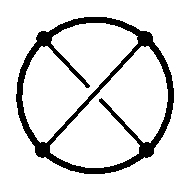
\includegraphics[height=2cm]{poscross.eps}}}  \quad &= \quad  s \,\,\vcenter{\hbox{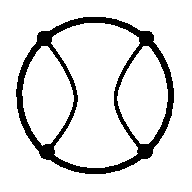
\includegraphics[height=2cm]{idresolution.eps}}}  + s^{-1} \,\, \vcenter{\hbox{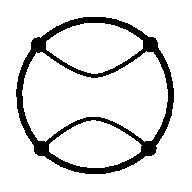
\includegraphics[height=2cm]{capcupresolution.eps}}}\\
\vcenter{\hbox{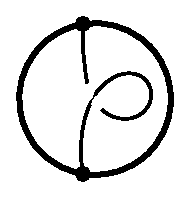
\includegraphics[height=2cm, keepaspectratio]{invvh.eps}}} \quad &= \quad -s^{3}\,\, \vcenter{\hbox{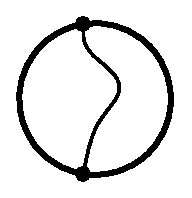
\includegraphics[height=2cm, keepaspectratio]{frameresolution.eps}}}. \notag
\end{align}

Given any 3-manifold, there is a natural map $\sk_s(M) \to K_s(M)$, which follows from the fact that the Kauffman bracket skein relations imply the Kauffman skein relations. If $M = F \times [0,1]$ for some surface $F$, then this is an algebra map.

%\PS{include Kauffman bracket skein relations}

The Frohman and Gelca presentation of the Kauffman bracket skein algebra uses the Chebyshev polynomials $T_n(x)$, which are uniquely characterized by the property $T_n(X+X^{-1}) = X^n + X^{-n}$. If $\xx \in \Z^2$ with $d(\xx) = k$, they defined an element $e_\xx \in K_s(T^2)$ by 
\[
e_\xx := T_k(\alpha_{\xx / k})
\]
where $\alpha_\xx$ is the simple closed curve of slope $\xx$.

\begin{lemma}
	The algebra map $\sk_s(T^2\times [0,1]) \to K_s(T^2\times [0,1])$ takes the generator $D_\xx$ to  $e_\xx$.
\end{lemma}
\begin{proof}
The closure of the symmetrizer $f_n$ in the annulus gets sent to the (closure of the) Jones-Wenzl idempotent in the Kauffman bracket skein algebra of the annulus, because both symmetrizers are uniquely determined by the way they absorb crossings and caps. Under the identification $K_s(S^1\times D^2) = \C[x]$, the closure of the Jones-Wenzl idempotent is sent to $S_n(x)$, the other version of the Chebyshev polynomial, which is defined by 
\[S_n(X+X^{-1}) = \frac{X^{n+1}-X^{-n-1}}{X-X^{-1}}.\]
All that is left to show is that the $S_n(x)$ and $T_n(x)$ satisfy the power series identity in Definition \ref{def:dk}, which we write as
\begin{equation*}
\sum_{k=1}^\infty \frac{T_k(x)}{k} t^k =\ln\left(1 + \sum_{j \geq 1} S_j(x) t^j\right).
\end{equation*}	
% \PS{add proof of this identity (later)} \AP{added a sketch}
Define different variants of  Chebyshev polynomials via $C_n^S(x/2):=S(x)$ and $2C_n^T(x/2):=T(x)$. The following two identities are well known (see, e.g. any book on special functions, or Wikipedia):
\begin{align*}
	\sum_{n \geq 0} C_n^S(x)t^n &= \frac{1}{1-2tx+t^2} \\
	\sum_{n \geq 1} C_n^T(x)\frac{t^n}{n} &= \ln \left( \frac{1}{\sqrt{1-2tx+t^2}} \right).
\end{align*}
The first identity implies 
\[
	1+\sum_{n \geq 1} S_n(x)t^n = \frac{1}{1-tx+t^2}.
\]
This implies the follow identities:
\begin{equation*}
	1+\sum_{n \geq 1} S_n(x)t^n  = \frac{1}{1-tx+t^2} = \left( \exp \left( \sum_{n \geq 1} C_n^T(x/2)\frac{t^n}{n} \right) \right)^2
	= \exp \left( \sum_{n \geq 1} 2 C_n^T(x/2)\frac{t^n}{n} \right).
\end{equation*}
This leads to the following, which completes the proof:
\begin{equation*}
\ln \left( 1+\sum_{n \geq 1} S_n(x)t^n \right) = \sum_{n \geq 1} 2 C_n^T(x/2)\frac{t^n}{n} = \sum_{n \geq 1} \frac{T_n(x)}{n} t^n.
\end{equation*} 
\end{proof}

Now let us recall the description of the Kauffman bracket skein algebra of the torus given by Frohman and Gelca.
\begin{theorem}[{\cite{FG00}}]\label{thm:fg}
	The Kauffman bracket skein algebra $K_s(T^2)$ has a presentation with generators $e_\xx$ and relations
	\begin{align}
	e_\xx e_\yy &= s^d e_{\xx + \yy} + s^{-d} e_{\xx-\yy}\label{eq:fgrel}\\
	e_{\xx} &= e_{-\xx}\notag
	\end{align}
	where $d = \det[\xx\,\yy]$.
\end{theorem}

A short computation using this presentation shows  the commutator identity
\begin{equation}\label{eq:fg}
[e_\xx, e_\yy] = (s^d-s^{-d}) (e_{\xx+\yy} - e_{\xx-\yy}).
\end{equation}
In other words, the relations we show for $D_\xx \in \sk(T^2)$ get sent to the relations in \eqref{eq:fg}, and the relations Frohman and Gelca showed in Theorem \ref{thm:fg} for the $e_\xx \in K_s(T^2)$ imply the relations in \eqref{eq:fg}. This shows our results are compatible with those of Frohman and Gelca.

\begin{remark}\label{rmk:sobig}
We emphasize that the algebra we describe is much bigger -- $\sk(T^2)$ has a linear basis given by unordered words in the $D_\xx$, while the Kauffman bracket skein algebra $K_s(T^2)$ has a linear basis given by the $e_\xx$ themselves. This happens because the Kauffman bracket skein relations allow all crossings to be removed from a diagram, so the algebra is spanned (over $R$) by curves without crossings. However, the more general Kauffman relations only allow crossings to be flipped, and not removed, which means the algebra is spanned (over $R$) by products of knots (which may have self-crossings). In particular, the relations \eqref{eq:fgrel} do not hold in the Kauffman skein algebra $\cd$.
\end{remark}

